%%%%%%%%%%%%%%%%%%%%%%%%%%%%%%%%%%%%%%%%%%%%%%%%%%%%%%%%%%%%%%%%%%%%%%%%
%     LaTeX source code to approximate a NIST Technical report
%	  Instructions for authors: tinyurl.com/techpubsnist 
%	DOI watermark will be added on final PDF
% 	Developed by K. Miller, kmm5@nist.gov 
%	Last updated: 22-January-2021
%%%%%%%%%%%%%%%%%%%%%%%%%%%%%%%%%%%%%%%%%%%%%%%%%%%%%%%%%%%%%%%%%%%
\documentclass[12pt]{book}

\usepackage{tcolorbox}
\usepackage{subcaption}
\usepackage{alltt}
\usepackage{svg}
\usepackage[scaled=0.6]{helvet}

\usepackage{xcolor}
\definecolor{color-uclm}{RGB}{176,8,55} % Adjust the RGB values as needed
\definecolor{mygreen}{rgb}{0,0.6,0}
\definecolor{mygray}{rgb}{0.5,0.5,0.5}
\definecolor{mymauve}{rgb}{0.58,0,0.82}

% Define a new tcolorbox environment for key concepts
\newtcolorbox{keyconceptbox}[1][]{ % Optional argument for title
  colback=blue!5!white, % Use the custom color
  colframe=blue, % Use the same color for the border
  fonttitle=\bfseries, % Title font
  title={#1}, % Title text
  rounded corners, % Set the radius for rounded corners
  boxrule=2pt % Border width
}

% Define a new tcolorbox environment for aclaraciones
\newtcolorbox{aclaracion}[1][]{ % Optional argument for title
  colback=red!5!white, % Use the custom color
  colframe=color-uclm, % Use the same color for the border
  fonttitle=\bfseries, % Title font
  title={#1}, % Title text
  rounded corners, % Set the radius for rounded corners
  boxrule=2pt % Border width
}

\usepackage{listings}

\lstnewenvironment{mycode}[1][]
{\lstset{#1}} % Options for the listings package
{}

\lstdefinestyle{mycodestyle}{
  backgroundcolor=\color{gray!10}, % Background color
  % Add other styling options as needed
}

\lstdefinestyle{cstyle}{
    language=C,
    basicstyle=\ttfamily,
    keywordstyle=\color{blue},
    commentstyle=\color{green!40!black},
    stringstyle=\color{red},
    numbers=left,
    numberstyle=\tiny,
    numbersep=5pt,
    frame=single,
    breaklines=true,
    breakatwhitespace=true,
    captionpos=b,
    showstringspaces=false,
    tabsize=4
}


\lstdefinestyle{verilogstyle}{
  language=Verilog, % Set the language to Verilog
  basicstyle=\ttfamily\small,
  commentstyle=\color{mygreen},
  keywordstyle=\color{blue},
  numberstyle=\tiny\color{mygray},
  stringstyle=\color{mymauve},
  breaklines=true,
  frame=single,
  numbers=left,
  showstringspaces=false
}


\usepackage{wrapfig}


% lcverbatim
\usepackage{fancyvrb,newverbs,xcolor}

%\setmonofont[Scale=0.8]{Courier New Bold}
\definecolor{cverbbg}{gray}{0.93}
\newenvironment{cverbatim}
 {\SaveVerbatim{cverb}}
 {\endSaveVerbatim
  \flushleft\fboxrule=0pt\fboxsep=.5em
  \colorbox{cverbbg}{\BUseVerbatim{cverb}}%
  \endflushleft
}
\newenvironment{lcverbatim}
 {\SaveVerbatim{cverb}}
 {\endSaveVerbatim
  \flushleft\fboxrule=0pt\fboxsep=.5em
  \colorbox{cverbbg}{%
    \makebox[\dimexpr\linewidth-2\fboxsep][l]{\BUseVerbatim{cverb}}%
  }
  \endflushleft
}
\newcommand{\ctexttt}[1]{\colorbox{cverbbg}{\texttt{#1}}}
\newverbcommand{\cverb}
  {\setbox\verbbox\hbox\bgroup}
  {\egroup\colorbox{cverbbg}{\box\verbbox}}
% lcverbatim

\usepackage{amsmath}
\usepackage{amsfonts}   % if you want the fonts
\usepackage{amssymb}    % if you want extra symbols
\usepackage{graphicx}   % need for figures
\usepackage{xcolor}
\usepackage{bm}
\usepackage{secdot}		
\usepackage{mathptmx}
\usepackage{float}
\usepackage[utf8]{inputenc}
\usepackage{textcomp}
\usepackage[hang,flushmargin,bottom]{footmisc} % footnote format
\usepackage{multirow}
\usepackage{tabularray}

\usepackage{titlesec}
\titleformat{\section}{\normalsize\bfseries}{\thesection.}{1em}{}	% required for heading numbering style
\titleformat*{\subsection}{\normalsize\bfseries}

\usepackage{tocloft}	% change typeset, titles, and format list of appendices/figures/tables
\renewcommand{\cftdot}{}	
\renewcommand{\contentsname}{Table of Contents}
\renewcommand{\cftpartleader}{\cftdotfill{\cftdotsep}} % for parts
\renewcommand{\cftsecleader}{\cftdotfill{\cftdotsep}}
\renewcommand\cftbeforesecskip{\setlength{4pt}{}}
\addtolength{\cftfignumwidth}{1em}
\renewcommand{\cftfigpresnum}{\figurename\ }
\addtolength{\cfttabnumwidth}{1em}
\renewcommand{\cfttabpresnum}{\tablename\ }
\setlength{\cfttabindent}{0in}    %% adjust as you like
\setlength{\cftfigindent}{0in} 

\usepackage{enumitem}         % to control spacing between bullets/numbered lists

\usepackage[numbers,sort&compress]{natbib} % format bibliography 
\renewcommand{\bibsection}{}
\setlength{\bibsep}{0.0pt}

\usepackage[hidelinks]{hyperref}
\hypersetup{
	colorlinks = true,
urlcolor ={blue},
citecolor = {.},
linkcolor = {.},
anchorcolor = {.},
filecolor = {.},
menucolor = {.},
runcolor = {.}
pdftitle={},
pdfsubject={},
pdfauthor={},
pdfkeywords={}
}
\urlstyle{same}

\usepackage{epstopdf} % converting EPS figure files to PDF

\usepackage{fancyhdr, lastpage}	% formatting document, calculating number of pages, formatting headers
\setlength{\topmargin}{-0.5in}
\setlength{\headheight}{39pt}
\setlength{\oddsidemargin}{0.25in}
\setlength{\evensidemargin}{0.25in}
\setlength{\textwidth}{6.0in}
\setlength{\textheight}{8.5in}

\usepackage{caption} % required for Figure labels
\captionsetup{font=small,labelfont=bf,figurename=Fig.,labelsep=period,justification=raggedright} 

% Fix for pdfTeX warning of form: … found PDF version <1.6>, but at most version <1.5> allowed
% https://tex.stackexchange.com/questions/52317/pdftex-warning-version-allowed
\pdfminorversion=7

%%%%%%%%%%% !!!!!! REQUIRED - FILL OUT METADATA HERE !!!!!!!! %%%%%%%%%%%%%%
%  	Report Number - fill in Report Number sent to you (see info below)
%   DOI Statement - fill in DOI sent to you 
%   Month Year - fill in Month and Year of Publication
%%%%%%%%%%%%%%%%%%%%%%%%%%%%%%%%%%%%%%%%%%%%%%%%%%%%%%%%%%%%%%%%%%%%%%%%%%%%%%%%%%%%%%
\newcommand{\pubnumber}{XXXX}
\newcommand{\DOI}{https://doi.org/10.6028/NIST.HB.XXXX}
\newcommand{\monthyear}{Month Year}
%%%%%%%%%%%%%%%%%%%%%%%%%%%%%%%%%%%%%%%%%%%%%%%%%%%%%%%%%%%%%%%%%%%%
%   	BEGIN DOCUMENT 
%%%%%%%%%%%%%%%%%%%%%%%%%%%%%%%%%%%%%%%%%%%%%%%%%%%%%%%%%%%%%%%%%%%%
\begin{document}
	\urlstyle{rm} % Format style of \url   

%%%%%%%%%%%%%%%%%%%%%%%%%%%%%%%%%%%%%%%%%%%%%%%%%%%%%%%%%%%%%%%%%%%%
%   Cover Page is REQUIRED and must contain the information 
%	displayed here, at a minimum. Additional artwork may be included 
%	(e.g., official project/conference logo, etc.).
%	Pub Number automated based on metadata
%%%%%%%%%%%%%%%%%%%%%%%%%%%%%%%%%%%%%%%%%%%%%%%%%%%%%%%%%%%%%%%%%%%%
\begin{titlepage}
\begin{flushright}
%%%%%%%%%%%%%%%%%%%%%%%%%%%%%%%%%%%%%%%%%%%%%%%%%%%%%%%%%%%%%%%%%%%%
% 	Automated based on metadata - delete if not applicable
%%%%%%%%%%%%%%%%%%%%%%%%%%%%%%%%%%%%%%%%%%%%%%%%%%%%%%%%%%%%%%%%%%%%
\LARGE{\textbf{Computadores Avanzados}}\\
\vfill
%%%%%%%%%%%%%%%%%%%%%%%%%%%%%%%%%%%%%%%%%%%%%%%%%%%%%%%%%%%%%%%%%%%%
%	Title 
%%%%%%%%%%%%%%%%%%%%%%%%%%%%%%%%%%%%%%%%%%%%%%%%%%%%%%%%%%%%%%%%%%%%
\Huge{\textbf{Manual de Verilog}}\\
    \vfill
%%%%%%%%%%%%%%%%%%%%%%%%%%%%%%%%%%%%%%%%%%%%%%%%%%%%%%%%%%%%%%%%%%%%
%	Authors - add complete list of authors, affiliations will be 
%   added on title page
%%%%%%%%%%%%%%%%%%%%%%%%%%%%%%%%%%%%%%%%%%%%%%%%%%%%%%%%%%%%%%%%%%%%
    \large Antonio Morán Muñoz\\
\vfill
%%%%%%%%%%%%%%%%%%%%%%%%%%%%%%%%%%%%%%%%%%%%%%%%%%%%%%%%%%%%%%%%%%%%
%	The DOI is automated based on metadata.	
%%%%%%%%%%%%%%%%%%%%%%%%%%%%%%%%%%%%%%%%%%%%%%%%%%%%%%%%%%%%%%%%%%%%
\normalsize Manual de Verilog\\
\vfill
%%%%%%%%%%%%%%%%%%%%%%%%%%%%%%%%%%%%%%%%%%%%%%%%%%%%%%%%%%%%%%%%%%%%
%	NIST LOGO - keep as-is
%%%%%%%%%%%%%%%%%%%%%%%%%%%%%%%%%%%%%%%%%%%%%%%%%%%%%%%%%%%%%%%%%%%%


\includegraphics[width=0.3\linewidth]{figs/esiiab-logo.jpg}\\ 
 
  
\end{flushright}
\end{titlepage}
\begin{titlepage}
%%%%%%%%%%%%%%%%%%%%%%%%%%%%%%%%%%%%%%%%%%%%%%%%%%%%%%%%%%%%%%%%%%%%
%	Title Page is REQUIRED
%%%%%%%%%%%%%%%%%%%%%%%%%%%%%%%%%%%%%%%%%%%%%%%%%%%%%%%%%%%%%%%%%%%%
\begin{flushright}
%%%%%%%%%%%%%%%%%%%%%%%%%%%%%%%%%%%%%%%%%%%%%%%%%%%%%%%%%%%%%%%%%%%%
%   Publication Series & Number - automated
%%%%%%%%%%%%%%%%%%%%%%%%%%%%%%%%%%%%%%%%%%%%%%%%%%%%%%%%%%%%%%%%%%%%
\LARGE{\textbf{Diseño Digital}}\\
\vfill 
%%%%%%%%%%%%%%%%%%%%%%%%%%%%%%%%%%%%%%%%%%%%%%%%%%%%%%%%%%%%%%%%%%%%
%	Title 
%%%%%%%%%%%%%%%%%%%%%%%%%%%%%%%%%%%%%%%%%%%%%%%%%%%%%%%%%%%%%%%%%%%%
\Huge{\textbf{Manual de Verilog}}\\
    \vfill
%%%%%%%%%%%%%%%%%%%%%%%%%%%%%%%%%%%%%%%%%%%%%%%%%%%%%%%%%%%%%%%%%%%%
%	Author Order and Grouping. Always identify the primary author/creator first (s/he does not have to be a NIST author). For publications with multiple authors, group authors by their organizational affiliation. The organizational groupings and the names within each grouping should generally be ordered by decreasing level of contribution.
%	For non-NIST authors, list their city and state below their organization name.
%	For NIST authors, include the Division and Laboratory names (but do not include their city and state).
%%%%%%%%%%%%%%%%%%%%%%%%%%%%%%%%%%%%%%%%%%%%%%%%%%%%%%%%%%%%%%%%%%%%
    \normalsize Antonio Morán Muñoz\\
     \textit{Instituto de Investigación en Informática (I3A)}\\
    \vfill
%%%%%%%%%%%%%%%%%%%%%%%%%%%%%%%%%%%%%%%%%%%%%%%%%%%%%%%%%%%%%%%%%%%%
%   DOI Statement - automated
%%%%%%%%%%%%%%%%%%%%%%%%%%%%%%%%%%%%%%%%%%%%%%%%%%%%%%%%%%%%%%%%%%%%
\normalsize Esta publicación está basada en la plantilla NIST Handbook de Overleaf\\
\vfill
%%%%%%%%%%%%%%%%%%%%%%%%%%%%%%%%%%%%%%%%%%%%%%%%%%%%%%%%%%%%%%%%%%%%
%   Date - Month and Year - automated
%%%%%%%%%%%%%%%%%%%%%%%%%%%%%%%%%%%%%%%%%%%%%%%%%%%%%%%%%%%%%%%%%%%%
\normalsize Septiembre 2023
\vfill
%%%%%%%%%%%%%%%%%%%%%%%%%%%%%%%%%%%%%%%%%%%%%%%%%%%%%%%%%%%%%%%%%%%%
%  Department of Commerce LOGO - leave as-is
%%%%%%%%%%%%%%%%%%%%%%%%%%%%%%%%%%%%%%%%%%%%%%%%%%%%%%%%%%%%%%%%%%%%	


\includegraphics[width=0.5\linewidth]{figs/logo-cooiiclm.png}\\ 
 \vfill
%%%%%%%%%%%%%%%%%%%%%%%%%%%%%%%%%%%%%%%%%%%%%%%%%%%%%%%%%%%%%%%%%%%%
%  Department of Commerce & NIST Leadership 
%	will be updated as changes occur
%%%%%%%%%%%%%%%%%%%%%%%%%%%%%%%%%%%%%%%%%%%%%%%%%%%%%%%%%%%%%%%%%%%%
\footnotesize Departamento de Sistemas Informáticos\\ 
%\textit{Gina M. Raimondo, Secretary}\\
\vspace{10pt}
Universidad de Castilla-La Mancha\\ 
%\hspace*{-3cm}\textit{James K. Olthoff, Performing the Non-Exclusive Functions and Duties of the Under Secretary of Commerce \\
%for Standards and Technology \& Director, National Institute of Standards and Technology}
\end{flushright}
\end{titlepage}
\begin{titlepage}
%%%%%%%%%%%%%%%%%%%%%%%%%%%%%%%%%%%%%%%%%%%%%%%%%%%%%%%%%%%%%%%%%%%%
%   Disclaimer/CODEN page - required
%%%%%%%%%%%%%%%%%%%%%%%%%%%%%%%%%%%%%%%%%%%%%%%%%%%%%%%%%%%%%%%%%%%%
\begin{flushright}
\footnotesize  Certain commercial entities, equipment, or materials may be identified in this document in order to describe an experimental procedure or concept adequately. Such identification is not intended to imply recommendation or endorsement by the National Institute of Standards and Technology, nor is it intended to imply that the entities, materials, or equipment are necessarily the best available for the purpose.\\ 

\vfill
%%%%%%%%%%%%%%%%%%%%%%%%%%%%%%%%%%%%%%%%%%%%%%%%%%%%%%%%%%%%%%%%%%%%
%   This secton automated - do not change
%%%%%%%%%%%%%%%%%%%%%%%%%%%%%%%%%%%%%%%%%%%%%%%%%%%%%%%%%%%%%%%%%%%%
\normalsize \textbf{National Institute of Standards and Technology Handbook \pubnumber\\ 
Natl. Inst. Stand. Technol. Handbook \pubnumber, \pageref{LastPage} pages (\monthyear)} \\
\vspace{12pt}
\textbf{This publication is available free of charge from: \DOI}
\vfill
\end{flushright}
\end{titlepage}
%%%%%%%%%%%%%%%%%%%%%%%%%%%%%%%%%%%%%%%%%%%%%%%%%%%%%%%%%%%%%%%%%%%%
%   Start front matter - page number starts with "i"
%%%%%%%%%%%%%%%%%%%%%%%%%%%%%%%%%%%%%%%%%%%%%%%%%%%%%%%%%%%%%%%%%%%%
\section*{Foreword}
\pagenumbering{roman}
\normalsize Delete if not applicable\\
\section*{Preface}
\normalsize Delete if not applicable\\
\section*{Abstract}
\normalsize Required\\
\section*{Key words}
\normalsize Required, alphabetized, separated by semicolon, and end in a period.\\
\pagebreak
%%%%%%%%%%%%%%%%%%%%%%%%%%%%%%%%%%%%%%%%%%%%%%%%%%%%%%%%%%%%%%%%%%%%
%   Table of Contents is required
% 	List of Tables & Figures required if more than 5 tables/figures
%%%%%%%%%%%%%%%%%%%%%%%%%%%%%%%%%%%%%%%%%%%%%%%%%%%%%%%%%%%%%%%%%%%%
\begin{center}
\tableofcontents
\listoftables
\listoffigures
\end{center}
\pagebreak
\section*{Glossary}
Delete if not applicable\\
\pagebreak
%%%%%%%%%%%%%%%%%%%%%%%%%%%%%%%%%%%%%%%%%%%%%%%%%%%%%%%%%%%%%%%%%%%%
%   Start body of text - page number starts with "1"
%%%%%%%%%%%%%%%%%%%%%%%%%%%%%%%%%%%%%%%%%%%%%%%%%%%%%%%%%%%%%%%%%%%%
\pagenumbering{arabic}
\section{Conmutación Segmentada}\label{sec:p01intro}\pagenumbering{arabic}

\subsection{Objetivo}\label{ssec:p01objetivo}

\normalsize Asimilar el funcionamiento de wormhole y comprender la utilidad de incluir canales virtuales
en el diseño de las redes de interconexión.


\subsection{Desarrollo}\label{ssec:p01desarrollo}

La práctica consiste en resolver una serie de cuestiones relacionadas con la técnica de
conmutación wormhole. Para realizar esta práctica se hará uso del simulador SimuRed, descrito en
el apéndice A. Debéis poner a cero los paquetes iniciales de precalentamiento o de relleno, para que
obtenga adecuadamente las estadísticas.

\begin{itemize}
    \item[\textbf{a)}] \textbf{Para comprobar la manera en la que se produce la transmisión de datos cuando se aplica wormhole, selecciona una topología toro 2D 4 × 4, con buffers con capacidad para 2 flits, paquetes de 3 flits (incluida la cabecera), retardos de 1 ciclo, encaminamiento determinista y un canal virtual; y simula la transferencia de 2 paquetes: uno enviado desde el nodo 0 al nodo 5 y otro enviado desde el nodo 2 también al nodo 5. Ambos envíos comienzan en el ciclo 0.}

    La única complejidad en este apartado es la de hacer una traza que recoja los paquetes que nos piden. Para ello, será necesario crear un fichero de texto con la extensión \verb|.trc| y en el incluir una línea por cada paquete que se quiera enviar (en el manual del simulador se explican con más detalle los campos que incluir en cada línea). El Listing \ref{lst:traza} muestra el resultado.

    \begin{mycode}[style=mycodestyle, caption={Traza a simular.}, label=lst:traza]
0 0 5
0 2 5
    \end{mycode}

    Durante la ejecución de la traza paso a paso, es interesante ver lo que ocurre cuando ambos paquetes compiten por los recursos en el nodo 1. En este caso, ante la colisión, el paquete proveniente del nodo 0 pasa primero, flit a flit. Además, cuando dicho paquete termina de salir de este nodo, el segundo paquete le sigue inmediatamente, pudiéndose apreciar la principal diferencia con \textit{Virtual Cut-Through}, ya que con esta técnica de conmutación, el paquete entero se bloquearía en el buffer del nodo 1 hasta que los buffers de entrada del nodo 5 estuviesen completamente libres, ya que la conmutación se realiza a nivel de paquete.

    \begin{keyconceptbox}[Wormhole]
        Es una técnica de conmutación en la que el control de flujo se ejerce sobre cada uno de los flits en los que se divide el mensaje, al contrario que en el \textit{Virtual Cut-Through}, en la que el control de flujo se lleva a cabo a nivel de paquete. Esto significa que el tamaño de los buffers se reduce mucho en wormhole, ya que sólo se tienen que asegurar los recursos para un flit, no para el paquete entero. La latencia viene dada por la siguiente fórmula:

        \begin{equation*}
        T_{WH} = D(t_r + t_s + t_w) + max(t_s,t_c)\left\lceil\frac{L}{W}\right\rceil
        \end{equation*}
        
    \end{keyconceptbox}

    \begin{keyconceptbox}[Toro]
        Es un tipo de topología de red directa y ortogonal. Pertenece a la familia de topologías $n$-cubo $k$-arias. En un toro, cada nodo está conectado con dos vecinos a lo largo de dos o más dimensiones. Un toro 2D 4x4 se podría visualizar como cuatro colgantes de perlas cerrados, con cuatro perlas cada uno. Estos cuatro colgantes estarían dispuestos verticalmente, de manera que cada perla estuviera en línea y conectada con la inmediatamente superior y la inferior. Además, cada perla de la cadena más superior, estaría conectada a la perla correspondiente de la cadena más inferior. Estas características, diferencian al toro de la malla, ya que los nodos situados en los extremos de esta, no están conectados entre sí.

        \vspace{10pt}

        \centering 	\fbox{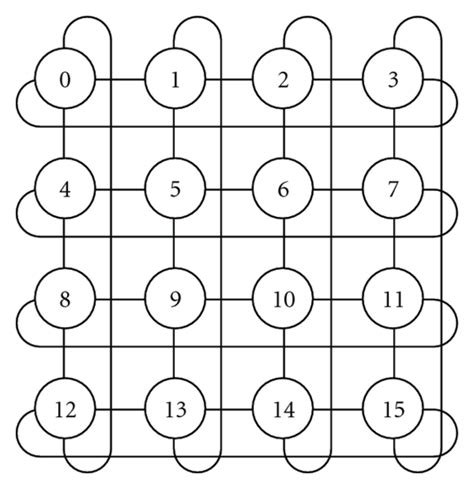
\includegraphics[width=0.5\linewidth]{figs/red-toroidal.jpeg}} \label{fig:red-toroidal}
    \end{keyconceptbox}

    \item[\textbf{b)}] \textbf{Para el ejemplo del apartado anterior, analiza los resultados estadísticos que se obtienen, explicando cada uno de ellos. Repite la misma simulación para otros tamaños de paquete y de buffer (8 y 32 flits, por ejemplo). Observa lo que ocurre y comenta los resultados (indica lo que ocurre cuando los paquetes deben usar el mismo canal o lo que pasa cuando el tamaño del paquete es mucho mayor que el del buffer).}

    Tras salir del cuadro de simulación interactiva, en el recuadro blanco de la pestaña de simulación se muestran las estadísticas de la simulación. A continuación se muestran los resultados obtenidos tras simular la traza del apartado anterior. Dentro de dichas estadísticas se incluyen diferentes tasas:

    \begin{itemize}
        \item Tasa de creación = nº total de flits / nº total de ciclos / nº total de nodos
        \item Tasa de envíos = nº total de flits / nº total de nodos
        \item Tasa de recepción = nº total de flits / nº total de ciclos / nº total de nodos
    \end{itemize}
    
    \begin{mycode}[style=mycodestyle]
--------------------------------------------
Item: 1, Variable: 0.3
--------------------------------------------
Ciclos: 14
Paquetes Generados: 2
Paquetes Enviados:  2
Paquetes Recibidos: 2
---------------------------------------
Tasa  Creacion (flits/ciclo/nodo): 0.0267857142857143
Tasa de  Envio (flits/ciclo/nodo): 0.375
Tasa Recepcion (flits/ciclo/nodo): 0.0267857142857143
---------------------------------------
Latencia Cabeza:                 10
Latencia Cabeza (sin bloqueos):  8
Latencia Paquete:                12
Desviacion Estandar:             2
Latencia Paquete (sin bloqueos): 10
Ciclos de Bloqueo en Red:        2
--------------------------------
Camino medio (nodos):        3
Camino medio (canales):      2
 

SIMULACION COMPLETADA CON EXITO.
Tiempo de simulacion: 0 h, 0 m, 3 s.
    \end{mycode}

    \textit{¿Qué ocurre cuando los paquetes deben usar el mismo canal?} Lo que ocurre es que se produce una situación de bloqueo, ya que para salir del nodo 1, solo existe un buffer de salida. Al llegar al mismo tiempo ambos paquetes, uno de ellos se tiene que bloquear para que el otro paquete use el buffer.
    
    \textit{¿Qué pasa cuando el tamaño del paquete es mucho mayor que el del buffer?} Lo que ocurre es que el paquete que usa primero el buffer, lo retiene durante más ciclos, aumentando a su vez los ciclos de bloqueo y, en definitiva, la latencia media de la comunicación.
 

    \item[\textbf{c)}] \textbf{¿Cuál es la diferencia de funcionamiento si está activado o no el adelantamiento en colas o buffers?}

    La diferencia es que cuando el adelantamiento en colas está activado, el flit que entre en una cola se colocará en la primera posición libre de esta, mientras que con el adelantamiento desactivado dicho flit se colocaría al final de la cola y tendría que atravesar todas las posiciones intermedias para llegar al comienzo de la cola. La consecuencia del adelantamiento de colas es que se reduce la latencia, pues se reducen el número de ``saltos'' que el paquete tiene que dar hasta llegar a su destino. Esta diferencia será más evidente cuanto mayor sea el tamaño del buffer.

    \item[\textbf{d)}] \textbf{Propón como deberías configurar el simulador para que funcionara como VCT. }
    
    VCT realiza la conmutación a nivel de paquete, por lo que un nodo no puede aceptar un paquete si no puede asegurar que, en caso de bloqueo, puede almacenar el mensaje entero. Por lo tanto, para simular VCT en el simulador, bastaría con incrementar el tamaño de las colas por encima del tamaño de los paquetes.

    \item[\textbf{e)}] \textbf{Reproduce una situación en la que se muestre cómo el uso de canales virtuales puede reducir la contención provocada por wormhole, y con ello aumentar la utilización de los canales.}
    
    Simplemente con aumentar el número de canales virtuales a dos, se aprecia la diferencia, en especial si el tamaño de los paquetes es muy grande. En este caso, el paso de los paquetes de un nodo a otro se lleva a cabo de manera multiplexada en el tiempo, ya que el cable que los une es compartido por ambos paquetes, a pesar de que los exista un buffer para cada paquete. De esta manera, cuando ambos paquetes llegan al buffer de salida, el envío a través del cable que conecta ambos nodos se realiza de manera alterna: en $t_i$ pasa pasa un flit de un paquete, y en $t_{i+1}$ pasa un flit del otro paquete. 

    Si en el simulador aumentamos el tamaño de los buffers y desactivamos el adelanto en colas, se aprecia mejor la alternancia (véase la Figura \ref{fig:canales-virtuales}).

    \begin{figure}[h] % Adjust the width as needed
      \centering
      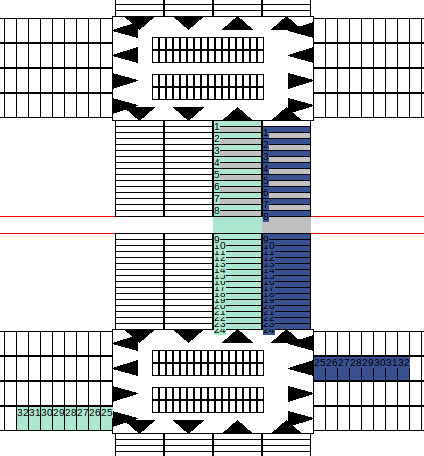
\includegraphics[width=0.3\textwidth]{figs/canales-virtuales.png} % Replace with your image filename
      \caption{Canales virtuales.}
      \label{fig:canales-virtuales}
    \end{figure}

\end{itemize}
\newpage
\section{Conmutación Segmentada}\label{sec:p02intro}\pagenumbering{arabic}

\subsection{Objetivo}\label{ssec:p02objetivo}

\normalsize Entender el problema de los deadlocks, y saber reproducirlos.

\subsection{Desarrollo}\label{ssec:p02desarrollo}

Se trata de crear una situación de interbloqueo (\emph{deadlock}) en diferentes topologías o en su caso analizar las circunstancias que lo impiden.

\begin{keyconceptbox}[Interbloqueo]
    También llamado bloqueo mortal (\emph{deadlock}), consiste en una dependencia de \emph{A} en \emph{B} y de \emph{B} en \emph{A} en el mismo instante de tiempo. Esto ocurre cuando, durante su recorrido, un recurso (e.g. un buffer) requerido por \emph{A} está siendo utilizado por \emph{B}. Al mismo tiempo, durante su recorrido, \emph{B} requiere del uso de un recurso que está siendo utilizado por \emph{A}. De esta manera, ninguno de los dos podrá avanzar, ya que dichos recursos no podrán ser liberados nunca.

    \vspace{10pt}

    \centering 	\fbox{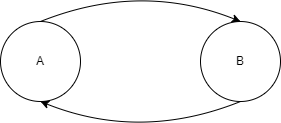
\includegraphics[width=0.5\linewidth]{figs/diagrama-interbloqueo.drawio.png}} \label{fig:diagrama-interbloqueo}
    
\end{keyconceptbox}

\begin{itemize}
    \item[\textbf{a)}] \textbf{Un caso muy sencillo se puede obtener en una red de interconexión con topología toro 2D, considerando canales unidireccionales.}

    Para obtener un interbloqueo en una dimensión, es conveniente (y para dimensiones de cuatro nodos, necesario) que los paquetes recorran el camino más largo posible. De esta manera, será más probable que ambos paquetes se encuentren en sus caminos. Asimismo, es necesario que ambos paquetes salgan de nodos situados a la mayor distancia posible entre ellos ya que, de lo contrario, con cuatro nodos se rompería cualquier ciclo posible. La Figura \ref{fig:interbloqueo-simured} muestra una situación de interbloqueo en la que el paquete A sale del nodo 0 al 1, y el paquete B del nodo 2 al 3. Véase que si hubiéramos lanzado el paquete B desde el nodo 1 al 2, se rompería el ciclo de dependencia, ya que el paquete A podría alcanzar el nodo 1 sin problemas.

    \begin{figure}[h] % Adjust the width as needed
      \centering
      \fbox{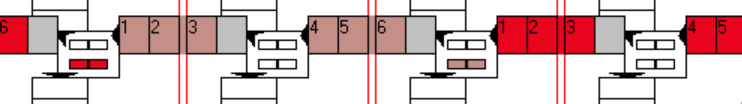
\includegraphics[width=0.9\textwidth]{figs/interbloqueo-zoom.png}} % Replace with your image filename
      \caption{Interbloqueo en Simured.}
      \label{fig:interbloqueo-simured}
    \end{figure}

    \item[\textbf{b)}] \textbf{Plantear casos más complejos que intervengan nodos de dos dimensiones distintas, utilizando la topología que consideréis oportuna y aplicando canales bidireccionales o unidireccionales. En su caso si no se consigue el bloqueo analizar las circunstancias que lo impiden.}\par
    \textbf{En todos los casos, se utilizará el simulador \emph{SimuRed}, descrito en el apéndice A.}

    En este caso el interbloqueo se tiene que dar de tal manera que todos los paquetes tengan que utilizar las dos dimensiones en su recorrido. Para ello, y en primer lugar, hay que utilizar un algoritmo de encaminamiento totalmente adaptativo, ya que de lo contrario se rompería cualquier ciclo. En segundo lugar, los canales tienen que ser bidireccionales. En tercer lugar, en este caso será necesario lanzar cuatro paquetes. Por último, la longitud del paquete debería ser mayor que el doble de la longitud de las colas. En este caso, para generar el interbloqueo, hay que lanzar los paquetes en cruz. El Listing \ref{lst:traza2b} muestra un ejemplo de traza que enviaría los paquetes en cruz. 

    \begin{mycode}[style=mycodestyle, caption={Traza para provocar un interbloqueo en dos dimensiones.}, label=lst:traza2b]
0 9 6
0 6 9
0 10 5
0 5 10
    \end{mycode}

    Al utilizar un algoritmo de encaminamiento determinista, es posible que no se produzca un interbloqueo a la primera. Por eso, es probable que se tengan que realizar varias ejecuciones con la misma traza hasta que aparezca. La Figura \ref{fig:interbloqueo-2d} muestra un posible interbloqueo en dos dimensiones usando Simured.

    \begin{figure}[h] % Adjust the width as needed
      \centering
      \fbox{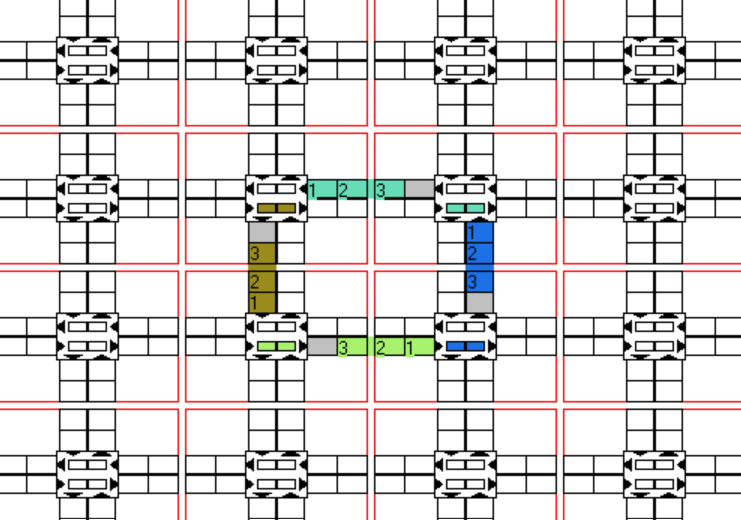
\includegraphics[width=0.7\textwidth]{figs/interbloqueo-2d.png}} % Replace with your image filename
      \caption{Interbloqueo en dos dimensiones.}
      \label{fig:interbloqueo-2d}
    \end{figure}

\end{itemize}
\newpage
\section{Encaminamiento determinista y adaptativo}\label{sec:p03intro}\pagenumbering{arabic}

\subsection{Objetivo}\label{ssec:p03objetivo}

\normalsize Comprobar y entender el funcionamiento de algoritmos de encaminamiento deterministas y
adaptativos.

\subsection{Desarrollo}\label{ssec:p03desarrollo}

\normalsize La práctica consiste en resolver una serie de  cuestiones relacionadas con el mecanismo de encaminamiento en redes de interconexión. Para realizar esta práctica se hará uso del simulador \emph{SimuRed}, descrito en el apéndice A.

\begin{itemize}
    \item [\textbf{a)}] \textbf{Reproduce una situación con la que se pueda observar el beneficio introducido por el encaminamiento adaptativo en lo que se refiere a nivel de  prestaciones de la red, comparándolo con el caso de encaminamiento determinista.}

    \textbf{Se trata de realizar una pequeña traza para alcanzar el objetivo, y observar mediante una simulación interactiva la evolución de los paquetes por la red.  Utilizar para ello el algoritmo de encaminamiento determinista y el totalmente adaptativo.}

    Para comprobar el beneficio del encaminamiento adaptativo frente al determinista es necesario crear una situación de congestión en la que varios paquetes hagan uso de los mismos recursos. De esta manera, se creará un cuello de botella en ese punto que el encaminamiento adaptativo será capaz de solventar y el determinista no. En este caso, se va a usar la traza mostrada en el Listing \ref{lst:traza3a}.

    \begin{mycode}[style=mycodestyle, caption={Traza para provocar congestión.}, label=lst:traza3a]
0 9 6
0 6 9
0 10 5
0 5 10
    \end{mycode}
    
    En la Figura \ref{fig:detvsadap} se puede ver el resultado de lanzar dicha traza con ambos encaminamientos. Como se puede ver la reducción en el número de ciclos requeridos para completar la simulación es notable cuando se emplea el algoritmo adaptativo. No obstante, hay que destacar que el encaminamiento totalmente adaptativo tomará dará lugar a diferentes resultados, pudiendo darse casos en que se produzca congestión como en el caso del encaminamiento determinista.

\begin{figure}[hbt]
  \centering
  \begin{subfigure}{0.48\textwidth}
    %\centering
    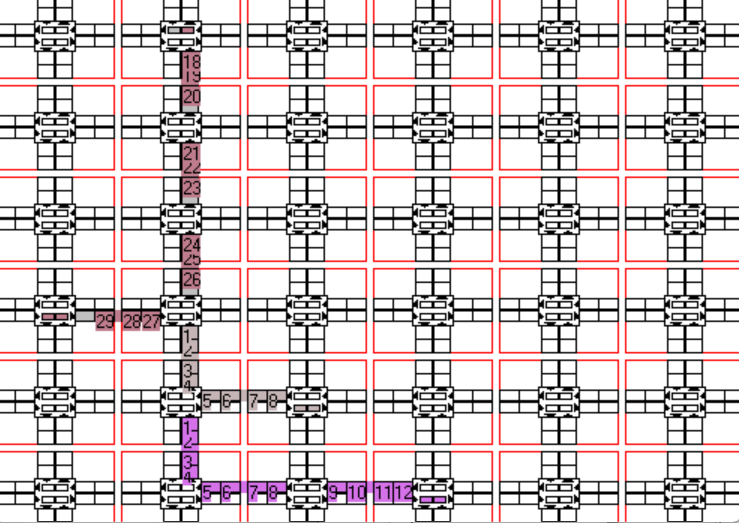
\includegraphics[width=\linewidth]{figs/congestion-simured.png}
    \caption{Encaminamiento determinista}
    %\label{fig:initial-bufferless}
  \end{subfigure}
  \hspace{0.25cm}
  \begin{subfigure}{0.48\textwidth}
    %\centering
    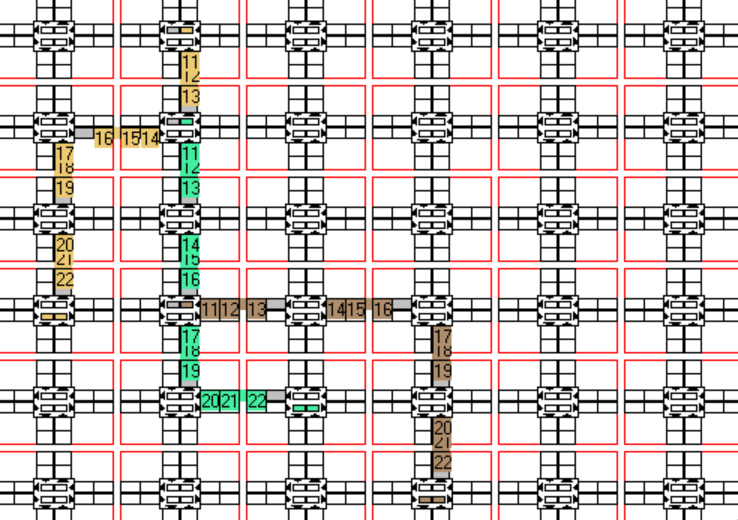
\includegraphics[width=\linewidth]{figs/adaptativo-simured.png}
    \caption{Encaminamiento adaptativo}
    %\label{fig:initial-bufferless}
  \end{subfigure}
  
  \vspace{1cm} % Add some vertical space
  
  \begin{subfigure}{0.48\textwidth}
    %\centering
    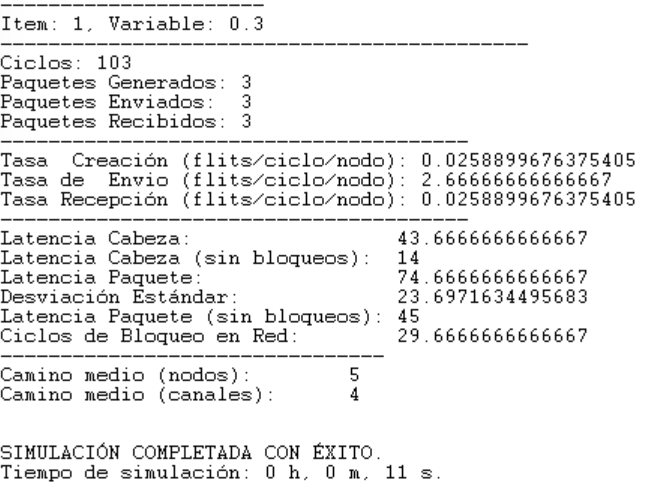
\includegraphics[width=\linewidth]{figs/determinista-estadisticas.png}
    \caption{Estadísticas encaminamiento determinista}
    %\label{fig:dropping}
  \end{subfigure}
  \hspace{0.25cm}
  \begin{subfigure}{0.48\textwidth}
    %\centering
    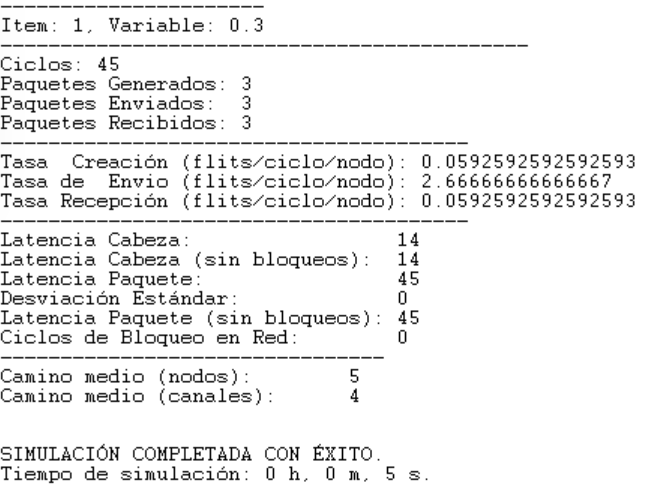
\includegraphics[width=\linewidth]{figs/adaptativo-estadisticas.png}
    \caption{Estadísticas encaminamiento adaptativo}
    %\label{fig:misrouting}
  \end{subfigure}
  \caption{Encaminamiento determinista vs adaptativo}
  \label{fig:detvsadap}
\end{figure}

    \item [\textbf{b)}] \textbf{Para comprobar las diferencias de una forma más clara entre los dos tipos de encaminamiento (en este caso determinista y el adaptativo de Duato), se realizará una evaluación más completa.}

    \textbf{Consistirá en obtener la latencia para diferentes tasas de inyección y comparar mediante las correspondientes gráficas los resultados para ambos algoritmos de encaminamiento. Un número recomendable de paquetes son $20000$ descartando, de cara a los resultados, del 5 al 10\% de los iniciales. Para este apartado utilizar la opción de guardar estadísticas en un fichero e ir acumulando los resultados en una misma gráfica para poder realizar las oportunas comparativas.}

    \item[\textbf{c)}] \textbf{Finalmente realizar una comparativa con diferente número de canales virtuales y justificar adecuadamente los resultados obtenidos.} 
    
\end{itemize}
\newpage
\section{Encaminamiento determinista y adaptativo}\label{sec:p03intro}\pagenumbering{arabic}

\subsection{Objetivo}\label{ssec:p03objetivo}

\begin{itemize}
    \item \normalsize Poner de manifiesto el problema de llevar datos compartidos a varias caches.
    \item \normalsize Comparar protocolos de coherencia basados en invalidación y basados en actualización.
\end{itemize} 

\subsection{Desarrollo}\label{ssec:p03desarrollo}

\normalsize Se trata de poner de manifiesto el problema denominado falsa compartición (false sharing). Esta situación se da cuando unos bloques de datos son compartidos por varios procesadores. Un procesador modifica un determinado dato que pertenece a un bloque dado. Otro procesador modifica otro dato distinto pero que pertenece al mismo bloque. El bloque es llevado a las caches de ambos procesadores y, si se usa un protocolo de coherencia basado en invalidación, se producirán elevadas tasas de fallos en cache y de transferencias de bloques.

Para realizar esta práctica el alumno debe usar el simulador SMPCache (apéndice B).

\begin{itemize}
    \item [\textbf{a)}] \textbf{El alumno debe crear trazas de accesos a memoria que reproduzcan esa situación. Para ello usará el código mostrado en el Listing \ref{lst:codigo}, el cual realiza una operación elemental sobre vectores que consiste en hacer una copia de un vector en otro. Dicha copia la realizan entre varios procesadores, repartiéndose por igual las componentes del vector. Para poder ver el efecto del problema de la falsa compartición, el alumno debe considerar al menos dos formas de hacer ese reparto: una que produzca el problema de la falsa compartición y otra que no.}

    \begin{mycode}[style=cstyle, caption={Código para realizar copia de vectores y generar trazas para SMPCache.}, label=lst:codigo]
// Programa que copia un vector en otro
// Genera trazas para el simulador SMPCache
#include <stdlib.h>
#include <stdio.h>
#include <string.h>

const int NUM = 1000; // Longitud del vector
const int N = 8;      // Maximo numero de procesadores
const int READ = 2;   // Lectura de datos
const int WRITE = 3;  // Escritura de datos
const int FETCH = 0;  // Captura de instrucciones

int n, i, proc;

// Funcion para repartir los datos entre los procesadores
int DisData(char key, int i) {
    int proc;
    switch (key) {
        // INSERTAR CODIGO
    }
    return proc;
}

// Funcion que escribe en un fichero un acceso a memoria.
// Parametros: fichero, tipo de acceso y direccion accedida
void WriteAccess(FILE *f, int type, void *address) {
    fprintf(f, "%d %p\n", type, address);
}

int main(int argc, char *argv[]) {
    char a[NUM], b[NUM]; // Vectors
    FILE *f[N]; // File per processor
    char filename[30];
    char key;
    
    if ((argc == 2) && (INSERTAR CODIGO)) {
        key = argv[1][0];
    } else {
        printf("Syntax: ...\n");
        exit(0);
    }

    for (n = 1; n <= N; n *= 2) {
        for (proc = 0; proc < n; proc++) {
            sprintf(filename, "traza%c%d_%d.prg", key, n, proc + 1);
            f[proc] = fopen(filename, "w");
        }
        for (i = 0; i < NUM; i++) {
            a[i] = b[i]; // Example operation
            proc = DisData(key, i);
            WriteAccess(f[proc], READ, &b[i]);  // Read b[i]
            WriteAccess(f[proc], WRITE, &a[i]); // Write to a[i]
        }
        for (proc = 0; proc < n; proc++) {
            fclose(f[proc]);
        }
    }
    return 0;
}
    \end{mycode}


    \textbf{Se deben hacer pruebas con 2, 4 y 8 procesadores, y por tanto se deben generar las trazas necesarias para cada uno de esos tres casos. Por ejemplo, cuando se simule un SMP con 4 procesadores son necesarios 4 ficheros de traza, uno para cada procesador. La configuración base del SMP será la dada por los siguientes parámetros:}

    \begin{itemize}
        \item \textbf{Protocolo de coherencia: MESI}
        \item \textbf{Procesadores: 8}
        \item \textbf{Arbitraje del Bus: LRU}
        \item \textbf{Tamaño de palabra: 8 bits}
        \item \textbf{Palabras por bloque: 128}
        \item \textbf{Bloques en la memoria: 8192}
        \item \textbf{Bloques en la cache: 64}
        \item \textbf{Correspondencia: Asociativa por conjuntos}
        \item \textbf{Conjuntos: 32 (2 vías)}
        \item \textbf{Reemplazo: LRU}
    \end{itemize}

    \textbf{Se debe tomar nota de los resultados que produce el simulador, y que son el número de transferencias de bloques en el bus y la tasa de fallos o aciertos de cache.}

    El código del Listing \ref{lst:codigo-solucion} es el que hay que incluir en la función \verb|DisData|. Los :

\begin{mycode}[style=cstyle, caption={Funcion para repartir los datos entre los procesadores.}, label=lst:codigo-solucion]
int DisData(char key, int i) {
    int proc;
    switch (key) {
        case 'C': 
            proc = (n * i) / NUM; /* Reparto por bloques */
            break;
        case 'I': 
            proc = i % n; /* Reparto ciclico */
            break;
    }
    return proc;
}
\end{mycode}

    También nos tenemos que asegurar de que se pasan los parámetros 'C' e 'I' al programa:

    \begin{mycode}[style=cstyle, caption={Comprobación de los parámetros del programa.}, label=lst:codigo-solucion2]
if ((argc == 2) && (argv[1][0]=='C' || argv[1][0]=='E')) {
	key = argv[1][0];
} else { 
	printf ("Sintaxis: C (Continuo) | E (entrelazado)\n");
	exit(0);
}
  \end{mycode}
	


    \item [\textbf{b)}] \textbf{Con las trazas generadas en el apartado anterior realiza una comparación de los protocolos MESI (invalidación) y Dragon (actualización). Varía el número de procesadores para realizar la comparación.}

    \item[\textbf{c)}] \textbf{Finalmente realizar una comparativa con diferente número de canales virtuales y justificar adecuadamente los resultados obtenidos.} 
    
\end{itemize}
\newpage
\section{Encaminamiento determinista y adaptativo}\label{sec:p03intro}\pagenumbering{arabic}

\subsection{Objetivo}\label{ssec:p03objetivo}

\subsection{Desarrollo}\label{ssec:p03desarrollo}


\begin{itemize}
    \item [\textbf{Ejercicio 1.}] \textbf{Extraer la topología de red a un fichero ”topologia.topo”, y dibujarla utilizando “InfiniBand-Graphviz”:}

    Para hacer este ejercicio, lo primero que hay que hacer es conectarse a CELLIA usando \verb|slurm|

    \item [\textbf{Ejercicio 2.}] \textbf{¿Qué topología de las vistas en clase hay construida en CELLIA? Anotar sus propiedades (nº de nodos, nº de switches, grado del switch, etc.)}

    \item[\textbf{Ejercicio 3.}] \textbf{Modificar el fichero “device\_list.c” para que
ofrezca más información acerca del HCA de un nodo.} 

    \item[\textbf{Ejercicio 4.}] \textbf{Modificar un programa con verbs para añadir
información acerca del uso de la red.} 
    
\end{itemize}
\newpage
\section{La dimensión temporal}
Verilog permite especificar un \emph{tiempo de demora} en \emph{asignaciones continuas}. Esto se hace incluyendo el carácter almohadilla (\#) y un número real después de la palabra clave \verb|assign|. El número real indica la demora en las unidades indicadas por la \emph{escala temporal}. También se puede especificar una demora en asignaciones procedurales. En este caso, la almohadilla y el número se colocan tras los símbolos \verb|<| o \verb|<=|. Para especificar la \emph{escala temporal}, se usa la directiva del compilador \verb|`timescale| con la siguiente sintaxis:

\begin{alltt}
\texttt{\`}timescale \emph{time-unit} / \emph{time-precision}
\end{alltt}

\emph{time-unit} indica la unidad que estará asociada con las demoras\footnote{e.g. si \emph{time-unit} es igual a $ns$, una demora de 2 se traducira a $2ns$.}. Por otro lado, \emph{time-precision} indica la granularidad con la que operará el simulador (sueles tener un valor de $ps$).
Estos valores serán tenidos en cuenta también por \emph{tareas y funciones del sistema} como \verb|$time|.

Otra manera de invocar una demora temporal dentro del \emph{código procedural} es usando la \hyperlink{delay_statement}{\emph{sentencia de demora}}, que es un \# seguido de un número. Es importante tener en cuenta que las demoras temporales serán tenidas en cuenta durante la simulación, pero no durante la síntesis. 
\newpage
\section{Simulación}

Una vez que la tenemos un modelo de Verilog con sintaxis y semántica correcta, se puede y debe utilizar un simulador para observar su operación.

El simulador opera comenzando en un \hyperlink{simulation_time}{\emph{tiempo de simulación}} de cero. En este punto, el simulador inicializa todas las señales a un valor por defecto de \verb|x|. A continuación, el simulador inicializa las señales o variables cuyos valores iniciales han sido declarados explícitamente. Tras esto, el simulador comienza la ejecución de las sentencias concurrentes del diseño.

\begin{aclaracion}[Aclaración]
    El simulador en realidad no puede ejecutar las sentencias concurrentes simultáneamente. Sin embargo, crea esa ilusión mediante el uso de una \hyperlink{event_list}{\emph{lista de eventos}} basados en tiempo. y una \hyperlink{sensitivity_matrix}{matriz de sensibilidad} basada en todas las listas de sensibilidad individuales.\\

    Cada sentencia concurrente se da lugar a un procesos software, mientras que una instanciación de módulo puede dar lugar a uno o más procesos. En tiempo de simulación cero, todos los procesos generados se planifican para ejecución, de los cuales se selecciona uno. La ejecución del código procedural se lleva a cabo secuencialmente. Si se ha especificado una demora, la ejecución del proceso se suspende. Cuando esto ocurre (o cuando el proceso se ha terminado de ejecutar) se selecciona otro proceso para su ejecución.\\

    Cuando todos los procesos se han ejecutado, se completa lo que se denomina un \hyperlink{simulation_cycle}{\emph{ciclo de simulación}}.
\end{aclaracion}

Cuando el simulador se encuentra una asignación no bloqueante sin demora, ésta se supone que se ejecuta en tiempo de simulación cero. No obstante, lo que ocurre realmente es que se planifica su ejecución para el tiempo de simulación actual al que se le suma una \hyperlink{delta_delay}{\emph{demora delta}}. 

Cada vez que un ciclo de simulación es completado, la lista de eventos es escaneada para buscar las señales que antes cambien. Debido a que algunos procesos pueden ser sensibles al cambio de señales, la matriz de sensibilidad indica, para cada señal, qué procesos tienen dicha señal en su lista de sensibilidad. Cada proceso que sea sensible a una señal, será planificado para que se ejecute en el siguiente ciclo de simulación. Este proceso se repite hasta que la lista de eventos queda vacía, momento en el cual la simulación termina.
\newpage
\section{Bancos de pruebas}
Un \hyperlink{test_bench}{\emph{banco de prueba}} especifica una secuencia de entradas que serán aplicadas por el simulador al modelo HDL que será probado. Dicho modelo puede ser un módulo Verilog o un diseño más grande. La entidad sujeta a las pruebas se denomina \hyperlink{unit_under_test}{\emph{unidad bajo prueba (UBP)}}.

En bancos de pruebas es frecuente emplear otro tipo de sentencia concurrente, el bloque \verb|initial|. Esta sentencia se ejecuta una sola vez, en tiempo de simulación cero. Al igual que el bloque \verb|always|, se puede incluir un bloque \verb|begin-end| para declarar el código procedural.

\begin{mycode}[style=verilogstyle, caption={Banco de prueba para un circuito detector de numeros primos.}, label=lst:programa5-10]
`timescale 1 ns / 100 ps

module Vrprime_tb1();
reg [3:0] Num;
wire Prime;

Vrprimed UUT (.N(Num), .F(Prime));

    initial begin: TB
        integer i;
        for (i = 0; i <= 15; i = i+1) begin #10 
            Num = i;
        end
endmodule
\end{mycode}

Los simuladores suelen generar un fichero que especifica las formas de onda que cada señal toma durante la simulación. Dicho fichero puede ser leído por aplicaciones específicas para su visualización. El correcto funcionamiento la UBP quedará a cargo del usuario, cuya función es interpretar si las formas de onda tienen sentido. Debido a que este proceso es tedioso, es conveniente formatear la salida del simulador para que sea más amigable. Para ello se pueden usar tareas del sistema como \verb|$write| o \verb|$display| para mostrar información que se considere útil por consola o, incluso, redirigirla a un fichero.

Hay situaciones en las que la combinación de entradas que una UBP puede recibir es tan elevada. En estos casos, puede no resultar factible para el diseñador examinar los resultados obtenidos para cada combinación de entradas. En estos casos, conviene escribir un \hyperlink{self-checking_test_beng}{banco de prueba autoevaluado}
\newpage
\section{Circuitos combinacionales}

\subsection{Decodificadores}
A pesar de que los decodificadores en Verilog suelen formar parte de diseños mayores, también se pueden definir y probar de manera aislada. Para diseñar un decodificador, existen las siguientes aproximaciones:

\begin{itemize}
    \item \emph{Estilo estructural.} Consistiría en definir la operación del decodificador mediante puertas lógicas. Esta aproximación daría lugar a un código difícil de leer y de mantener.
    \item \emph{Estilo de flujo de datos.} Se define el comportamiento del circuito mediante sentencias de asignación contínua. El Listing \ref{lst:programa6-2} muestra un posible diseño.

\begin{mycode}[style=verilogstyle, caption={Estilo de flujo de datos.}, label=lst:programa6-2]
module decodificador_2a4(input a0, 
                   input a1, 
                   input en, 
                   output y0, 
                   output y1, 
                   output y2, 
                   output y3);
    assign y0 = en ? ({a1,a0} == 2'b00) : 0;
    assign y1 = en ? ({a1,a0} == 2'b01) : 0;
    assign y2 = en ? ({a1,a0} == 2'b10) : 0;
    assign y3 = en ? ({a1,a0} == 2'b11) : 0;
endmodule
\end{mycode}
    
    \item \emph{Estilo conductual.} Se modela el circuito por medio de código prodedural. El Listing \ref{lst:programa6-3} muestra un posible diseño.

\begin{mycode}[style=verilogstyle, caption={Estilo conductual.}, label=lst:programa6-3]
module decodificador_2a4(input a0, 
                   input a1, 
                   input en, 
                   output reg y0, 
                   output reg y1, 
                   output reg y2, 
                   output reg y3);

    always @(*) begin
        if(en) begin
            {y3,y2,y1,y0} = 0
            case ({a1,a0})
                2'b00: y0 = 1;
                2'b00: y1 = 1;
                2'b00: y2 = 1;
                2'b00: y3 = 1; 
                default: {y3,y2,y1,y0} = 0;
            endcase
        end
    end
    
endmodule
\end{mycode}

Una vez diseñado el circuito, es hora de probarlo.

\begin{mycode}[style=verilogstyle, caption={Banco de pruebas del decodificador.}, label=lst:programa6-4, mathescape]
`timescale 1 ns / 1 ps
module tb_decodificador_2a4();

    // declaracion de tipos de datos
    reg a0_p, a1_p, en_p;
    wire y0_p, y1_p, y2_p, y3_p;
    integer i, errores;
    reg [3:0] resultado_esperado;

    decodificador_2a4 UBP (.a0(a0_p),
                     .a1(a1_p),
                     .en(en_p),
                     .y0(y0_p),
                     .y1(y1_p),
                     .y2(y2_p),
                     .y3(y3_p)
                    );
    initial begin
        errors = 0;
        for(i = 0; i < 8; i++) begin
            {en, a0, a1} = i;
            #10;
            resultado_esperado = 4'b0000;
            if(en) resultado_esperado[{a1,a0}] = 1'b1;
            if ({y3,y2,y1,y0} !== resultado_esperado) begin
                errores = errores + 1;
            end
        end
        $\$$display("Test completado con $\%$d errores", errores);
    end
    
endmodule
\end{mycode}

Si la compilación con \verb|iverilog| ha sido correcta, el banco de pruebas debería mostrar 0 errores.

\subsubsection{Tipos de decodificadores}

\begin{itemize}
    \item \emph{Decodificadores binarios.} Un decodificador binario $n$-a-$2^n$ es un circuito con una entrada de $n$ bits y una salida activa de las $2^n$ totales.
    \item \hyperlink{seven-segment_decoder}{\emph{Decodificadores de siete segmentos.}} Estos circuitos tienen una entrada de 4 bits (Decimal Codificado en Binario) y una salida de 1 bit para cada segmento del LCD.
\end{itemize}

\subsection{Codificadores binarios}
Un codificador binario es un circuito que hace la acción opuesta al decodificador binario. Si un decodificador binario convierte un código de $n$ bits en otro de $m$ bits, el codificador binario correspondiente debe ser capaz de transformar el código de $m$ bit en el de $n$ bits.

\subsection{Multiplexores}
Una operación muy común en diseño digital es escoger una fuente de datos entre varias para transferirla a su destino a través de un medio compartido, como un bus. Esta operación es tan común que tiene su propio nombre, \hyperlink{multiplexing}{\emph{multiplexación}} o \emph{mux} para abreviar.

Una definición más precisa de multiplexador es la de \textit{conmutador digital que conecta los datos de 1 entre $n$ fuentes a una sola salida}. Para ello, al multiplexor hay que conectarle una entrada que permita hacer una selección entre $n$ fuentes. La anchura de este entrada de selección tendra que ser $log_2(n)$, donde $n$ es el número de fuentes.



\subsection{Demultiplexores}
Los demultiplexores son los dispositivos digitales que realizan la operación opuesta a los multiplexores, es decir, conectar una entrada (de $b$ bits) a una de entre $n$ destinos/salidas.
\end{itemize}
\newpage
\chapter{Circuitos secuenciales}

Aunque hemos comentado con profusión los circuitos combinacionales, lo que realmente impera en la práctica son los circuitos secuenciales. Mientras que hemos visto que en los circuitos combinacionales la salida depende exclusivamente de los valores de las entradas en el momento actual, en los circuitos secuenciales se tienen los valores de las entradas en el pasado. Por ejemplo, si tenemos un ventilador con diferentes velocidades y queremos aumentarla, tenemos que saber algo más aparte de una entrada que indique el incremento de la velocidad. Es decir, tendría que haber un estado que nos indique la velocidad actual del sistema para saber cómo incrementar la velocidad. Es aquí donde entran en juego las \emph{máquinas de estado.}

\section{Máquinas de estado.}

El funcionamiento de un sistema como el ventilador puede ser conceptualizada como un conjunto de estados interrelacionados, es decir, una \hyperlink{state-machine}{máquina de estados.} El estado de un circuito secuencial puede definirse como ``una colección de \emph{variables de estado} cuyos valores en cualquier instante contienen toda la información acerca del pasado necesaria para predecir el comportamiento del circuito en el futuro'' \textcolor{red}{CITAR LIBRO DE HERERT HELLERMAN DIGITAL COMPUTER SYSTEM PRINCIPLES DE 1967}. No obstante, son necesarias más cosas aparte de variables de estado, por ejemplo, se necesita saber hacia qué estado. Este no solo dependerá del valor de las entradas del sistema, sino del estado en el que se encuentre en ese momento. En el ejemplo del ventilador, si activamos la señal de incremento de la velocidad y nos encontramos en el estado \emph{VELOCIDAD\_MEDIA}, el circuito se moverá al estado \emph{VELOCIDAD\_ALTA}. Por el contrario, para la misma entrada, si el circuito se encontrara en el estado \emph{VELOCIDAD\_BAJA}, éste cambiaría a \emph{VELOCIDAD\_MEDIA}. Como el númerod de estados de un sistema no es infinito, las máquinas de estado (y los circuitos secuenciales en general) se suelen conocer también por el nombre de \emph{máquinas de estados finitos.}

En los circuitos secuenciales cobra gran importancia el \emph{reloj}, ya que los cambios entre estados deben llevarse a cabo de manera sincronizada. En la mayoría de sistemas, el cambio de estado se lleva a cabo en los \hyperlink{edge}{\emph{flancos}} del reloj, o \hyperlink{active_edge}{\emph{flancos activos/gatillo}}, ya sea de subida o de bajada (aunque es más frecuente en el de subida). Una señal de reloj es \hyperlink{active_high}{\emph{activa en alto}} si los cambios de estado se producen en el flanco de subida, o \hyperlink{active_low}{\emph{activa en bajo}} si los cambios se llevan a cabo en el flanco de bajada. Este tipo de relojes debe estár activo, funcionando a una frecuencia dada y regular, mientras el circuito esté activo. Esta señal de reloj con frecuencia es generada por un oscilador de cristal de cuarzo, cuya frecuencia varía dependiendo del circuito en el que se integre.

Otro elemento a tener en cuenta en los circuitos secuenciales es el de \hyperlink{flip-flop}{biestable}. Estos son elementos con memoria, que permiten mantener el valor de las variables de estado, entre otras cosas. Un biestable se puede implementar por medio de un \hyperlink{feedback_sequential_circuit}{\emph{circuito secuencial retroalimentado}}, en el cual un bucle de retroalimentación se incluye en el circuito secuencial para añadir memoria al sistema. Hay multitud de tipos de biestables:

\begin{itemize}
    \item \emph{Biestable SR.}
    \item \emph{Biestable JK.}
    \item \emph{Biestable D.}
    \item \emph{Biestable T.}
\end{itemize}

\subsection{Estructura de las máquinas de estado}

La mayoría de máquinas de estado actuales son \hyperlink{clocked_synchronous_state_machine}{\emph{máquinas de estado sincronizadas por reloj}} que usan biestables D disparados por flanco. Son sincronizados por reloj porque todos los biestables están conectados a la misma señal de reloj, cambiando al mismo tiempo su estado en respuesta a los flancos del reloj. Las Figuras \ref{fig:mef-mealy} y \ref{fig:mef-moore} muestran la estructura general de una máquina de estados finitos de Mealy y de Moore, respectivamente. Ambas tienen en común una \emph{memoria de estado}, que está constituida por un conjunto de $n$ biestables que almacenan el estado del circuito. A estos biestables se les conecta una \emph{señal de reloj} común, the tal manera que el estado sólo cambia en los \emph{tics} del reloj. El \emph{tic} (se podría definir como el instante en el que cambia el estado) depende del tipo de biestable usado. Por ejemplo, para los biestables que se activan en el flanco de subida, el tic es el flanco de subida del reloj. El estado siguiente de la máquina de estados viene determinado por la \emph{lógica del estado siguiente} que es función del estado actual y las entradas. En cambio, la \emph{lógica de salida} depende del tipo de circuito del que se trate. En las máquinas de estados finitos de Mealy, la lógica de salida viene determinada por las entradas y el estado actual.

\begin{figure}[h]
    \centering
    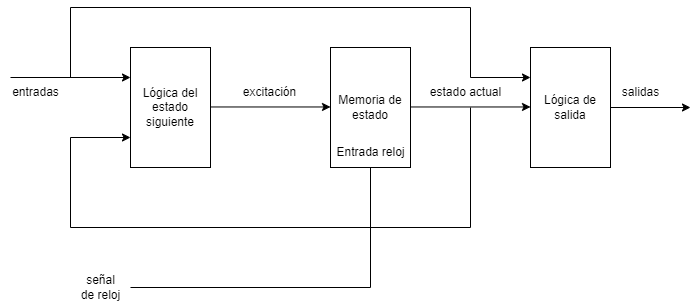
\includegraphics[width=\textwidth]{figs/mef-mealy.drawio.png}
    \caption[short]{Máquina de estados finitos de Mealy.}
    \label{fig:mef-mealy}
\end{figure}

En cambio, en una máquina de estados finitos de Moore, la lógica de salida viene determinada exclusivamente del estado actual.

\begin{figure}[h]
    \centering
    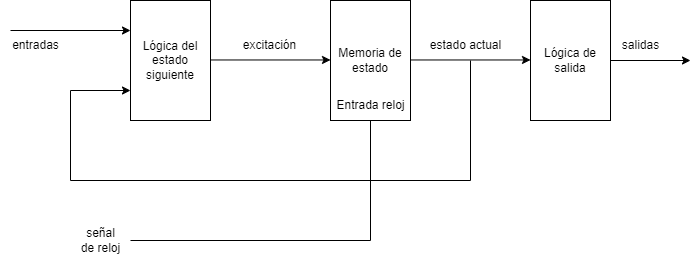
\includegraphics[width=\textwidth]{figs/mef-moore.drawio.png}
    \caption[short]{Máquina de estados finitos de Moore.}
    \label{fig:mef-moore}
\end{figure}

Como se puede observar en los diagramas, la única diferencia entre ambos tipos de modelos radica en cómo se generan las salidas. 

En el diseño de circuitos de gran velocidad es necesario que las salidas estén disponibles lo antes posible. Por ello, en ocasiones se codifican las variables de estado para que sirvan de salida también. Este tipo de diseño se denomina \hyperlink{output-coded_state_assignment}{\emph{asignación de estados codificada en salidas}}. En este caso la salida del circuito consiste en \verb|wires|. Otra manera de abordar el diseño de una máquina de estados es haciendo que la salida durante un periodo de reloj dependa de la salida en el periodo de reloj anterior. Esto se denomina \hyperlink{pipelined_outputs}{\emph{salida por etapas}} y se consigue uniendo otra etapa de memoria, llamada \emph{memoria de salida por etapas}, a las salidas del circuito.

\subsection{Temporización de las máquinas de estados}

\textcolor{red}{POR HACER}

\section{Diseño de máquinas de estado con tablas de estado}

\textcolor{red}{POR HACER (pag. 455)}

\section{Diseño de máquinas de estado con diagramas de estado}

\textcolor{red}{POR HACER (pag. 472)}

\section{Diseño de máquinas de estado con Verilog}

Para explicar el diseño de máquinas de estados vamos a partir de las siguientes especificaciones:

Diseña una máquina de estados síncrona con reloj con dos entradas, A y B, y una salida Z que es 1 si:

\begin{itemize}
    \item A tiene el mismo valor que en los dos tics de reloj previos.
    \item B vale uno tras la última vez que la primera condición fue cierta.
\end{itemize}

Si las condiciones no se cumplen, Z vale 0.

Para visualizar mejor estas condiciones, lo mejor es comenzar describiendo una tabla de estados y salidas. La Tabla \ref{tab:tabla-salidas-estados} muestra el resultado sobre el cual vamos a trabajar para escribir el código en Verilog.

\begin{table}
    \centering
    \begin{tblr}{
      row{2} = {c},
      row{3} = {c},
      row{4} = {c},
      row{5} = {c},
      row{6} = {c},
      row{7} = {c},
      cell{1}{2} = {c=4}{c},
      cell{8}{2} = {c=5}{c},
      hline{1,9} = {-}{},
      hline{2} = {2-5}{},
      hline{8} = {2-6}{},
    }
                        & \textbf{\textit{AB}} &                      &                      &                      &                     \\
    \textbf{\textit{S}} & \textbf{\textit{00}} & \textbf{\textit{01}} & \textbf{\textit{11}} & \textbf{\textit{10}} & \textbf{\textit{Z}} \\
    INIT                & A0                   & A0                   & A1                   & A1                   & 0                   \\
    A0                  & OK0                  & OK0                  & A1                   & A1                   & 0                   \\
    A1                  & A0                   & A0                   & OK1                  & OK1                  & 0                   \\
    OK0                 & OK0                  & OK0                  & OK1                  & A1                   & 1                   \\
    OK1                 & A0                   & OK0                  & OK1                  & OK1                  & 1                   \\
                        & S*                   &                      &                      &                      &                     
    \end{tblr}

    \caption{Tabla de salidas y estados}
    \label{tab:tabla-salidas-estados}
    \end{table}

El correspondiente módulo en Verilog se compondrá de cinco secciones:

\begin{enumerate}
    \item La declaración de las entradas, salidas y variables internas al módulo.
    \item Sentencias \verb|parameter| para asignar las variables de estado a su nombre.
    \item Un primer bloque \verb|always| para crear la memoria de estado.
    \item Un segundo bloque \verb|always| para definir el comportamiento del estado siguiente.
    \item Un tercer bloque \verb|always| para definir la lógica de salida.
\end{enumerate}

El código en Verilog resultante se muestra en el Listing \ref{lst:maquina-estado-verilog}.

\begin{mycode}[style=verilogstyle, caption={Máquina de estado en Verilog.}, label=lst:maquina-estado-verilog]
module mef (
            // reloj y reset
            input clk,
            input rst,

            // entradas
            input A,
            input B,

            // salidas (como vamos a usar codigo procedural, hay que declarar la salida como reg)
            output reg Z
           );

// senales internas
reg estado, estado_siguiente;

// asignacion de variables de estado a parametros
parameter [2:0] INIT = 3'b000;
                A0 = 3'b001;
                A1 = 3'b010;
                OK0 = 3'b011;
                OK1 = 3'b100;

// comportamiento del estado siguiente
always @(*) begin
    case(estado)
        INIT: if (A == 0) estado_siguiente = A0;
              else estado_siguiente = A1;
        A0: if (A == 0) estado_siguiente = OK0;
            else estado_siguiente = A1;
        A1: if (A == 0) estado_siguiente = A0;
            else estado_siguiente = OK1;
        OK0: if (A == 0) estado_siguiente = OK0;
             else if ((A == 0) && (B == 1)) estado_siguiente = OK1;
             else estado_siguiente = A1;
        OK1: if ((A == 0) && (B == 0))             estado_siguiente = A0;
        else if ((A == 0) && (B == 1)) estado_siguiente = OK0;
        else estado_siguiente = OK1;
        default: estado_siguiente = INIT;
    endcase
end

// logica de salida
always @(estado) begin
    case(estado)
        INIT: Z = 0;
        A0: Z = 0;
        A1: Z = 0;
        OK0: Z = 1;
        OK1: Z = 1;
        default: Z = 0;
    endcase
end

// memoria de estado
always @(posedge clk) begin
    if(rst)
        estado <= 0;
    else
        estado <= estado_siguiente;
end
endmodule
\end{mycode}

En el Listing \ref{lst:mef-verilator} se muestra el banco de pruebas en C++ \footnote{En la documentación oficial, este fichero en C++ que sirve de banco de pruebas, se denomina "wrapper" (lo cual se podría traducir como envoltorio, ya que envuelve la instancia del modelo de la UBP generada por Verilator).}. En dicho banco de pruebas vemos cómo se instancia un objeto de la UBP (\verb|Vmef *dut = new Vmef;|). Dicho objeto es generado con Verilator mediante el siguiente comando.

\begin{lcverbatim}
verilator -Wall --trace -cc <nombre-de-UBP>.sv
\end{lcverbatim}

Lo que hace dicho comando es leer el código en Verilog/SystemVerilog (en este caso SystemVerilog) y lo compila en un modelo en C++. Dicho modelo consta de una serie de ficheros \verb|.cpp| y \verb|.h| que se alojan dentro del directorio \verb|obj_dir| situado en la ruta desde la cual se ejecutó el comando.

\begin{mycode}[style=verilogstyle, caption={Banco de pruebas en C++ que se simula con Verilator.}, label=lst:mef-verilator]
    #include <stdlib.h>
    #include <iostream>
    #include <bitset>
    #include <verilated.h>
    #include <verilated_vcd_c.h>
    //#include <verilated_dpi.h>
    #include "Vmef.h"
    #include "svdpi.h"
    #include "Vmef__Dpi.h"
    
    #define ESTADOS 5
    char estado = 0;
    vluint64_t tiempo = 0;
    int errores = 0;
    
    using namespace std;
    
    // funciones
    void reset(Vmef *dut, VerilatedVcdC *m_trace);
    void tic(Vmef *dut, VerilatedVcdC *m_trace);
    void prueba_estado(Vmef *dut, VerilatedVcdC *m_trace, int a, int b, int init);
    void comprueba(const string salida, const string esperado, const string prueba, int i, int j);
    
    // DPI
    extern void sv_method();
    
    int main(int argc, char** argv, char** env) {
        // instanciamos la UBP
        Vmef *dut = new Vmef;
    
        Verilated::scopesDump();
    
        // set the scope
        const svScope scope = svGetScopeFromName("TOP.mef");
        assert(scope);
        svSetScope(scope);
    
        // activamos la generacion de traza
        Verilated::traceEverOn(true);
        VerilatedVcdC *m_trace = new VerilatedVcdC;
        dut->trace(m_trace, 5);
        m_trace->open("waveform.vcd");
    
        // reseteamos la UBP
        reset(dut, m_trace);
    
        // PRUEBAS 
        // generamos un tic
        tic(dut, m_trace);
    
        // INIT
        prueba_estado(dut, m_trace, 0, 0, 0);
        // A0
        prueba_estado(dut, m_trace, 0, 0, 1);
        // A1
        prueba_estado(dut, m_trace, 0, 0, 2);
        // OK0
        prueba_estado(dut, m_trace, 0, 0, 3);
        // OK1
        prueba_estado(dut, m_trace, 0, 0, 4);
    
        // FIN PRUEBAS
        cout << "El numero de errores totales es " << errores << "\n\n";
    
    
        m_trace->close();
        delete dut;
        exit(EXIT_SUCCESS);
    }
    
    void reset(Vmef *dut, VerilatedVcdC *m_trace){
        dut->rst = 1;
        tic(dut, m_trace);
        dut->rst = 0;
        tic(dut, m_trace);
    }
    
    void tic(Vmef *dut, VerilatedVcdC *m_trace){
        dut->clk = 0;
        dut->eval();
        // volcamos 
        m_trace->dump(tiempo);
        tiempo++;
        dut->clk = 1;
        dut->eval();
        // volcamos 
        m_trace->dump(tiempo);
        tiempo++;
    
    }
    
    void prueba_estado(Vmef *dut, VerilatedVcdC *m_trace, int a, int b, int inicial){
        int i,j, entrada = 0;
        int intEst, intEst2;
        int contador = 0;
        string estado_prueba = "INIT"; 
        string estado = "INIT", esperado = "INIT"; 
    
        // mostramos el estado al entrar en la funcion
        std::cout << "\n\n---------------------------------------";
        std::cout << "\nEl estado al entrar en la funcion es " << estado << '\n';
        std::cout << "---------------------------------------";
        
        // for anidado para probar diferentes combinaciones de entrada
        for(i=0; i<2; i++){
            for(j=0; j<2; j++){
                dut->A = 0;
                dut->B = 0;
                // inicializamos el estado
                reset(dut, m_trace);
                // nos movemos al estado que queremos probar
                switch(inicial){
                    case 0: reset(dut, m_trace);
                            tic(dut, m_trace);
                            break;
                    case 1: dut->A = 0; 
                            tic(dut, m_trace);
                            break;
                    case 2: dut->A = 1; 
                            tic(dut, m_trace);
                            break;
                    case 3: dut->A = 0; 
                            tic(dut, m_trace);
                            dut->A = 0; 
                            tic(dut, m_trace);
                            break;
                    case 4: dut->A = 1; 
                            tic(dut, m_trace);
                            dut->A = 1;
                            tic(dut, m_trace);
                            break;
                    default: estado = "INIT";
                             tic(dut, m_trace);
                }
    
                // comprobamos que el estado inicial es el correcto 
                std::bitset<3> est(sv_get_estado());
                intEst = static_cast<int>(est[7]) ? (est.to_ulong() - 256) : est.to_ulong();
    
                switch(intEst){
                    case 0: estado_prueba = "INIT"; break;
                    case 1: estado_prueba = "A0"; break;
                    case 2: estado_prueba = "A1"; break;
                    case 3: estado_prueba = "OK0"; break;
                    case 4: estado_prueba = "OK1"; break;
                    default: estado_prueba = "INIT";
                }
    
                std::cout << "\n---------------------------------------\n";
                std::cout << "Estado inicializado a " << estado_prueba << '\n';
                std::cout << "---------------------------------------" << '\n';
    
    
                // calculamos el estado esperado
                switch(intEst){
                    case 0: if((i == 0) && (j == 0)){
                                    esperado = "A0";
                                 } else if ((i == 0) && (j == 1)){
                                     esperado = "A0";
                                 } else if ((i == 1) && (j == 0)){
                                     esperado = "A1";
                                 } else if ((i == 1) && (j == 1)) {
                                     esperado = "A1";
                                 } else esperado = "INIT";
                                 break;
                    case 1: if((i == 0) && (j == 0)){
                                    esperado = "OK0";
                                 } else if ((i == 0) && (j == 1)){
                                     esperado = "OK0";
                                 } else if ((i == 1) && (j == 0)){
                                     esperado = "A1";
                                 } else if ((i == 1) && (j == 1)) {
                                     esperado = "A1";
                                 } else esperado = "INIT";
                                 break;
                    case 2: if((i == 0) && (j == 0)){
                                    esperado = "A0";
                                 } else if ((i == 0) && (j == 1)){
                                     esperado = "A0";
                                 } else if ((i == 1) && (j == 0)){
                                     esperado = "OK1";
                                 } else if ((i == 1) && (j == 1)) {
                                     esperado = "OK1";
                                 } else esperado = "INIT";
                                 break;
                    case 3: if((i == 0) && (j == 0)){
                                    esperado = "OK0";
                                 } else if ((i == 0) && (j == 1)){
                                     esperado = "OK0";
                                 } else if ((i == 1) && (j == 0)){
                                     esperado = "A1";
                                 } else if ((i == 1) && (j == 1)) {
                                     esperado = "OK1";
                                 } else esperado = "INIT";
                                 break;
                    case 4: if((i == 0) && (j == 0)){
                                    esperado = "A0";
                                 } else if ((i == 0) && (j == 1)){
                                     esperado = "OK0";
                                 } else if ((i == 1) && (j == 0)){
                                     esperado = "OK1";
                                 } else if ((i == 1) && (j == 1)) {
                                     esperado = "OK1";
                                 } else esperado = "INIT";
                                 break;
                    default: esperado = "INIT";
                }
    
                
                // asignamos las combinaciones de entradas a dicho estado
                //std::cout << '\n' << "("<< estado_prueba << ") A = " << i << "\tB = " << j << '\n';
                //std::cout << "---------------------------------------" << '\n';
                dut->A = i;
                dut->B = j;
                tic(dut, m_trace);
    
               // comprobamos que el estado final es el correcto 
                std::bitset<3> est2(sv_get_estado());
                intEst2 = static_cast<int>(est2[7]) ? (est2.to_ulong() - 256) : est2.to_ulong();
    
                switch(intEst2){
                    case 0: estado = "INIT"; break;
                    case 1: estado = "A0"; break;
                    case 2: estado = "A1"; break;
                    case 3: estado = "OK0"; break;
                    case 4: estado = "OK1"; break;
                    default: estado = "INIT";
                }
    
                comprueba(estado, esperado, estado_prueba, i, j);
    
                contador++;
            }
        }
    }
    
    void comprueba(const string salida, const string esperado, const string prueba, int i, int j){
        if(salida.compare(esperado) != 0){
            cout << "\nEl resultado es erroneo, fracasado";
            std::cout << "\n---------------------------------------\n";
            std::cout << "A=" << i << " B=" << j << " -> " << salida << " != " << esperado << ", inutil mas que inutil." << '\n';
            std::cout << "---------------------------------------" << '\n';
    
            errores++;
        }
    }
\end{mycode}

\section{Otros elementos de lógica secuencial}
A parte de los ya mencionados biestables-D, usados para almacenar el estado de las máquinas de estados finitos, hay otros tipos de elementos de almacenamiento más apropiados para situaciones que no requieran de máquinas de estados finitos. Uno de estos elementos son los \emph{latches}. Estos permiten almacenar información basada en el nivel de una entrada de control con la mitad del coste que un \hyperlink{edge-triggered_flip-flop}{\emph{biestable disparado por flanco}} en términos de área del circuito. A continuación, se mostrarán algunos elementos usados en lógica secuencial por complejidad creciente.

\subsection{Biestable}
A pesar de que se ha mencionado el biestable D en secciones anteriores, no se ha llegado a explicar en que consiste. El biestable D es una evolución del biestable\footnote{En este caso, biestable se traduce al inglés como bistable, mientras que los biestables que se verán más adelante se traducen como flip-flops.}, que consiste en un par de \hyperlink{inverter}{\emph{inversores}} dispuestos de tal manera que forman un \emph{bucle de retroalimentación}. Estos biestables son los más simples y tienen dos salidas, Q y Q\_L, pero no tienen entradas (véase la Figura \ref{fig:biestable}).

\begin{wrapfigure}{o}{0.4\textwidth}
	\centering
	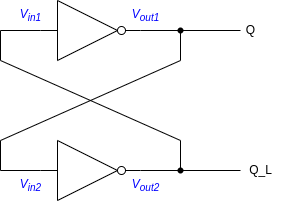
\includegraphics[width=0.35\textwidth]{figs/biestable.drawio.png}
	\caption{Biestable.}
	\label{fig:biestable}
\end{wrapfigure}

El biestable se llama así, porque el análisis digital muestra que tiene dos estados estables. Si Q es ALTO, entonces Q\_L es BAJO, lo cual refuerza el estado de Q. De esta manera tenemos dos estados estables, ALTO y BAJO. Lo mismo ocurre cuando Q es BAJO, ya que esto causa que Q\_L sea ALTO, lo que refuerza que Q sea BAJO. Al no disponer de ningún elemento de control o que nos permita cambiar el estado, al iniciar el biestable, este genera aleatoriamente el estado y se mantiene invariable para siempre.

\textcolor{red}{¿HABLAR DE METAESTABILIDAD AQUÍ?}

\subsection{Latches y biestables}
La diferencia entre latch y flip-flop es que mientras el latch refleja inmediatamente en la salida los cambios en la entrada, los flip-flops solo reflejan este cambio en los tics de reloj. A continuación se explican las diferentes variantes de latches y flip-flops.

\subsubsection{Latch S-R}

Los \hyperlink{sr_latch}{\emph{latch S-R}} son el circuito secuencial más simple que se puede construir y que tenga entradas de control. Se puede construir con dos puertas NOR de dos entradas (véase la Figura \ref{fig:latch-sr}). 

\begin{wrapfigure}{o}{0.4\textwidth}
    \centering
    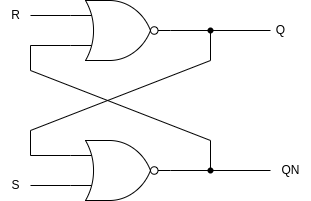
\includegraphics[width=0.35\textwidth]{figs/latch-sr.drawio.png}
    \caption{Latch S-R.}
    \label{fig:latch-sr}
\end{wrapfigure}

La 'S' y la 'R' vienen del inglés \emph{set} y \emph{reset}, y son las señales de control del circuito. Las salidas se denominan 'Q' y 'QN' y no tienen por qué ser una el complemento de la otra, a pesar de que normalmente en la mayoría de las aplicaciones lo suele ser. Por ejemplo, como se observa en la Figura \ref{fig:wave-latch-sr2}, si S y R valen 1 en el mismo instante de tiempo, las salidas cambian ambas a 0. Además, si se niegan tanto S como R al mismo tiempo, el circuito entra en un estado de metaestabilidad, haciendo el siguiente estado de las salidas impredecible. No obstante, si las entradas se niegan en instantes diferentes, las salidas retienen el estado anterior. Esto otorga al circuito su capacidad de almacenamiento.

\begin{figure}[h]
    \centering
  
    \begin{subfigure}[b]{0.35\textwidth}
      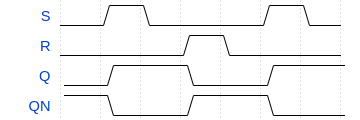
\includegraphics[width=\textwidth]{figs/wavedrom-latch-sr.png}
      \caption{Operación normal de un latch S-R.}
      \label{fig:wave-latch-sr1}
    \end{subfigure}
    \hfill
    \begin{subfigure}[b]{0.55\textwidth}
      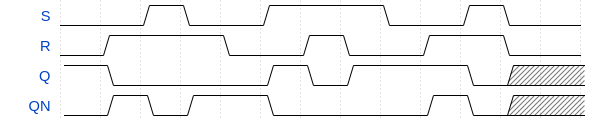
\includegraphics[width=\textwidth]{figs/wavedrom-latch-sr2.png}
      \caption{Operación anómala cuando 'S' y 'R' son afirmados a la vez.}
      \label{fig:wave-latch-sr2}
    \end{subfigure}
  
    \caption{Diagrama de ondas de un latch S-R}
    \label{fig:wave-latch-sr}
\end{figure}

\subsubsection{Latch $\overline{\text{S}}$-$\overline{\text{R}}$}
Los \emph{latch $\overline{S}$-$\overline{R}$} funcionan de manera similar a los anteriores, con la diferencia de que las entradas S y R son activas a nivel bajo. A diferencia de los latch S-R, estos pueden ser construidos a partir de puertas NAND. Debido a que las puertas NAND ofrecen ciertas ventajas sobre las NOR, en términos de velocidad y tamaño, estos latches suelen utilizarse más en cirtos contextos.

\subsubsection{Latch D}

\begin{wrapfigure}{o}{0.45\textwidth}
    \centering
    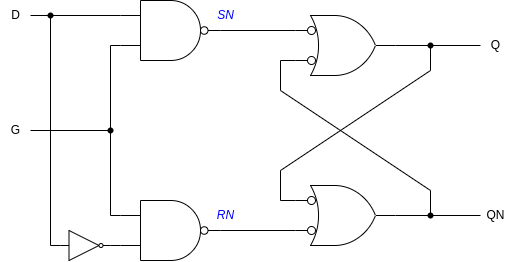
\includegraphics[width=0.4\textwidth]{figs/latch-d.drawio.png}
    \caption{Latch D.}
    \label{fig:latch-d}
\end{wrapfigure}

A pesar de que tanto el latch S-R como el $\overline{S}$-$\overline{R}$ pueden almacenar información, éstos se usan más en respuestas a ciertos cambios de condiciones del sistema que requieren reseteos. Para el almacenamiento de bits de información se utilizan otra clase de circuitos, que se verán a continuación. El primero de ellos es el \emph{latch D}.

Como se puede ver en la Figura \ref{fig:latch-d}, el latch D se construye sobre un latch $\overline{\text{S}}$-$\overline{\text{R}}$ al que se añaden dos puertas NAND con dos entradas: D, que es el dato que se quiere almacenar; y G, que es una señal de control que evita que se produzca la situación en la que tanto $\overline{\text{S}}$ como $\overline{\text{R}}$ sean afirmadas, dando lugar a metaestabilidad. De esta manera, 
\newpage
\section{Glosario}

\begin{itemize}
    \item \hypertarget{delay_statement}{Sentencia de demora} \emph{(delay statement)}.
    \item \hypertarget{simulation_time}{Tiempo de simulación} \emph{(simulation time)}.
    \item \hypertarget{event_list}{Lista de eventos} \emph{(event list)}.
    \item \hypertarget{sensitivity_matrix}{Matriz de sensibilidad} \emph{(sensitivity matrix)}.
    \item \hypertarget{simulation_cycle}{Ciclo de simulación} \emph{(simulation cycle)}.
    \item \hypertarget{test_bench}{Banco de prueba} \emph{(test bench)}.
    \item \hypertarget{unit_under_test}{Unidad bajo prueba} \emph{(unit under test (UUT))}.
    \item \hypertarget{seven-segment_decoder}{Decodificador de siete segmentos} \emph{(seven-segment decoder)}.
    \item \hypertarget{multiplexing}{Multiplexación} \emph{(multiplexing)}.
    \item \hypertarget{threestate_device}{Dispositivo triestado} \emph{(three-state device)}.
    \item \hypertarget{threestate_driver}{Conductor triestado} \emph{(three-state driver)}.
    \item \hypertarget{threestate_enable}{Habilitación triestado} \emph{(three-state enable)}.
    \item \hypertarget{priority_encoder}{Codificador con prioridad} \emph{(priority encoder)}.
    \item \hypertarget{IDLE}{OCIOSA} \emph{(IDLE)}.
    \item \hypertarget{comparator}{Comparador} \emph{(comparator)}.
    \item \hypertarget{magnitude_comparator}{Comparador de magnitudes} \emph{(magnitude comparator)}.
    \item \hypertarget{half_adder}{Semisumador} \emph{(half adder)}.
    \item \hypertarget{full_adder}{Sumador completo} \emph{(full adder)}.
    \item \hypertarget{ripple_adder}{Sumador con propagación} \emph{(ripple adder)}.
    \item \hypertarget{carry-lookahead_adder}{Sumador con anticipación de acarreo} \emph{(carry-lookahead adder)}.
    \item \hypertarget{group-ripple_adder}{Sumador con propagación grupal} \emph{(carry-ripple adder)}.
    \item \hypertarget{group-lookahead_adder}{Sumador con anticipación de acarreo grupal} \emph{(group-lookahead adder)}.
    \item \hypertarget{substractor}{Restador} \emph{(substractor)}.
    \item \hypertarget{shifter}{Desplazador} \emph{(shifter)}.
    \item \hypertarget{rotator}{Rotador} \emph{(rotator)}.
    \item \hypertarget{barrel_shifter}{Desplazador en barril} \emph{(barrel shifter)}.
    \item \hypertarget{state_machine}{Máquina de estados} \emph{(state-machine)}.
\end{itemize}
\newpage

%%%%%%%%%%%%%%%%%%%%%%%%%%%%%%%%%%%%%%%%%%%%%%%%%%%%%%%%%%%%%%%%%%%%
%   Figure references are “Fig. X��.
% 	“Figure X�� is used at beginning of sentence. 
% 	Figures should appear after they are mentioned in the text.
%	Figures must have embedded alternate text or “alt text�� in order 
%	to comply with Section 508 accessibility standards. 
%%%%%%%%%%%%%%%%%%%%%%%%%%%%%%%%%%%%%%%%%%%%%%%%%%%%%%%%%%%%%%%%%%%%
\section*{Acknowledgments}
\noindent Delete if not applicable\\
%%%%%%%%%%%%%%%%%%%%%%%%%%%%%%%%%%%%%%%%%%%%%%%%%%%%%%%%%%%%%%%%%%%%
%   Acknowledgments not required
%%%%%%%%%%%%%%%%%%%%%%%%%%%%%%%%%%%%%%%%%%%%%%%%%%%%%%%%%%%%%%%%%%%%

\section*{References}
\addcontentsline{toc}{section}{References}
\bibliographystyle{techpubs}
\nocite{*}
\bibliography{References}

%%%%%%%%%%%%%%%%%%%%%%%%%%%%%%%%%%%%%%%%%%%%%%%%%%%%%%%%%%%%%%%%%%%%
%   Please use the techpubs BibTeX style when compiling bibliography, or follow the instructions on tinyurl.com/techpubsnist to format your .bib / .bbl file appropriately.
%%%%%%%%%%%%%%%%%%%%%%%%%%%%%%%%%%%%%%%%%%%%%%%%%%%%%%%%%%%%%%%%%%%%

\section*{Appendix A: Supplemental Materials}
\addcontentsline{toc}{section}{Appendix A: Supplemental Materials}
Brief description of supplemental files\\

\section*{Appendix B: Change Log}
\addcontentsline{toc}{section}{Appendix B: Change Log}
If updating document with errata, detail changes made to document – delete if not applicable. \\

\end{document}
